\chapter{Novel approach to Classification in Imbalanced Datasets}\label{newapproach}
In previous chapter, we discussed approaches that improve classification for imbalanced datasets. We concluded that sampling and bagging techniques represent interesting approaches, as they can be applied to any classifier without the need to change them. Although especially synthetic samplers are promising (since they help to avoid overfitting), their implementation in imbalanced datasets is difficult. This is because the lack of data forces them to make some assumptions. As a result, these samplers will have worse performance when the posed assumptions do not hold or interfere with assumptions of the classifiers. We discuss this problem in section~\ref{rnd-intro}. In order to avoid this problem, we propose a new approach for classification in section~\ref{rnb-approach} that takes the assumptions of sampler and classifier into account. For this reason, a new sampler is introduced and explained in section~\ref{rnb-implementation}. Afterwards, this sampler is used in a specific setup such that all the posed assumptions are met and validated. We discuss the implications of this setup in section~\ref{rnb-implication} and show how the proposed approach allows reducing the variance in some situations. Finally, we formulate a conclusion in section~\ref{rnb-conclusion}.


\section{Introduction}\label{rnd-intro}
In the previous chapter we discussed how several techniques allow to improve the recognition rate of the minority class in imbalanced datasets. We also discussed that elegant solutions are mainly to be found in the use of ensembles and sampling techniques, since they do not require alterations in the base classifier. Experiment results in chapter~\ref{Experiments} show that these techniques indeed improve classifier performance. However, the results also show that one particular (synthetic) sampler, namely SMOTE, yields a performance degrade in many classifiers. The idea behind this observation is that when posed assumptions do not hold or interfere with the ones of the applied classifier, synthetic samplers such as SMOTE performs worse. For example, SMOTE assumes that the minority data are forming clusters of at least \(k\) instances. It then generates synthetic samples based on the existing within-cluster variance. When these assumptions do not hold, SMOTE will increase (rather than decrease) the existing level of noise. Moreover, experiments in chapter~\ref{Experiments} show that SMOTE significantly reduces the performance in a Naive Bayes classifier. This is probably related to the fact that SMOTE does not maintain the separate feature distributions.  Hence, we can conclude that the introduction of synthetic samplers in imbalanced datasets is a risky strategy. Another danger regarding synthetic samplers is that they often rely on feature interactions in order to approximate the minority distribution. Since the minority class data size is small, many of the captured feature interactions are very unreliable. Moreover, when the amount of features is large, most of these interactions are not even present in the training data. Hence, it is reasonable to mistrust the occurring feature interactions, and to impose feature independency in the minority dataset. The result is that by applying this technique, we can obtain samples that perfectly match the assumptions of a Naive Bayes classifier. In the next section, we discuss the approach of this technique.


\section{Approach}\label{rnb-approach}
In order to impose feature independency in the minority samples, we propose the following (synthetic) sampling scheme. Over-sample the minority distribution by creating (synthetic) instances where the feature values are bootstrapped independently from their original minority feature distribution. We call this sampler the \textbf{Naive Bayes Sampler} (NBS). We can say that NBS generates synthetic instances by randomly selecting (with replacement) feature values from their resp (minority class) prior distributions. The effect of NBS is illustrated in figure~\ref{fig:NBS}. Since NBS generates samples that are feature independent, they can best be used to train a Naive Bayes classifier (which assumes maximum conditional independence). Moreover, since the generated samples are influenced by a randomization process, the use of a bagging ensemble is favoured in order to decrease the variance over the estimates. Hence, we can summarize the proposed approach as follows:


\begin{enumerate}
\item \textbf{Over-sampling}: Create \textit{K} new (training) samples by copying the majority data, and creating \(o \times n_{minority}\) synthetic minority examples by bootstrapping from the individual feature values in the original minority dataset. The parameter \(o\) is defined by forehand and describes the oversample ratio.
\item \textbf{Bagging}: Train a Naive Bayes classifier on each separate generated training sample. These \textit{K} classifiers are then used to form a bagging ensemble.
\item \textbf{Prediction}: Test data is predicted by averaging the votes of the individual classifiers in the classifier ensemble.
\end{enumerate}

Since the disscussed approach introduces randomization in a Naive Bayes classifier by bootstrapping over feature-values, we call this approach \textbf{Random Naive Bayes by Feature-value Bootstrapping} (RNB-FvB). The experiment results of this approach can be found in section~\ref{exp-rnb}.







%-------------------------------------------------------------------------------------------------------------------
% IMPLEMENTATION
%-------------------------------------------------------------------------------------------------------------------
\section{Implementation}\label{rnb-implementation}
The following paragraphs explain in detail how this bootstrapping can be applied to nominal and numeric features.

Boostrapping nominal feature values is achieved by assigning feature values to synthetic instances by bootstrapping from their prior distribution. With other words, if \(N\) instances in training bag $B$ belong to class \(i\) and have feature value $v$ (out of $p$ possible feature values) for a given feature, the probability of selecting that feature value for an artificial object of class $i$ equals:

\begin{eqnarray}
&& P(v_i|B)=\frac{N_{iv}}{\sum_{j=1}^p{N_{ij}}}
\end{eqnarray}

Note that we also consider \textit{missing values} as a possible feature value.

\begin{figure}[h]
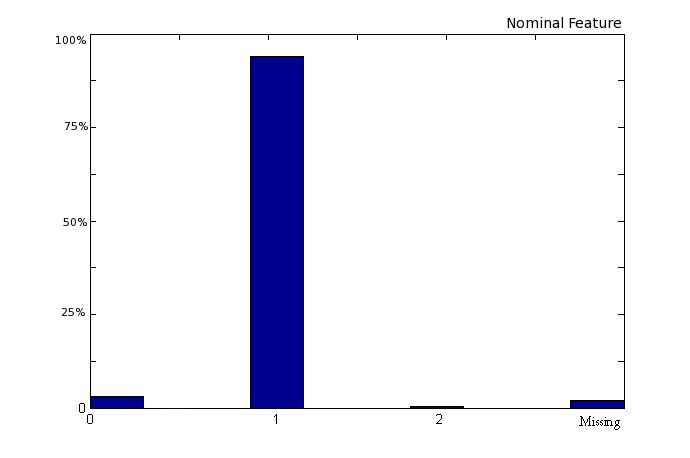
\includegraphics[scale=0.65]{img/nominalEst.png}
\caption{Bootstrapping nominal features}
\end{figure}

Bootstrapping numeric feature values is applied by a slightly more advanced technique. First, mean and variance of the prior distribution are estimated using Maximum Likelihood Estimation. These parameters are then used to generate new feature values along the prior (Gaussian) distribution. In order to avoid invalid feature values (for example when numeric features can only take positive values), their range of validity is defined. When an invalid feature value is then selected, it is assigned a new feature value according to the uniform distribution over the defined range. Hence, the original Gaussian distribution is augmented by a uniform distribution and only exists over the defined range.

\begin{landscape}
\begin{figure}[h]
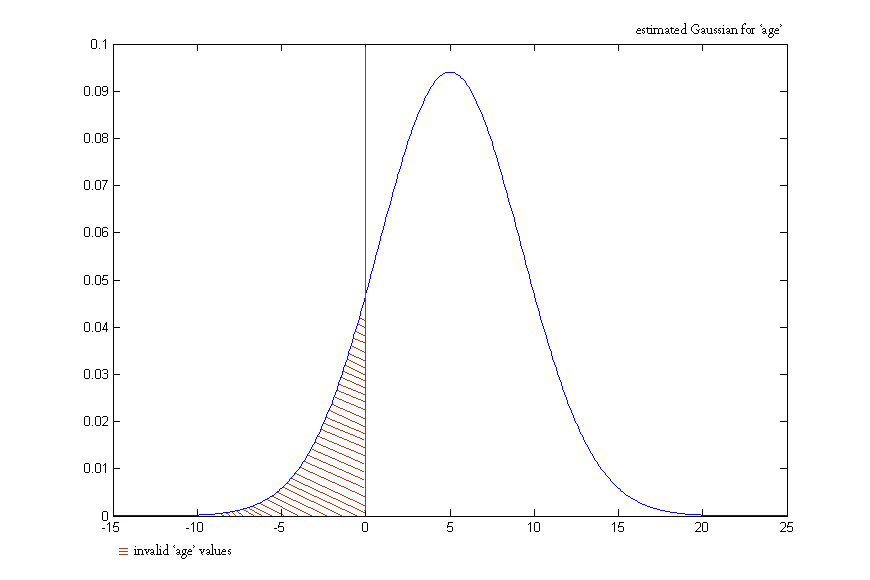
\includegraphics[scale=0.55]{img/AgeRegress.png} 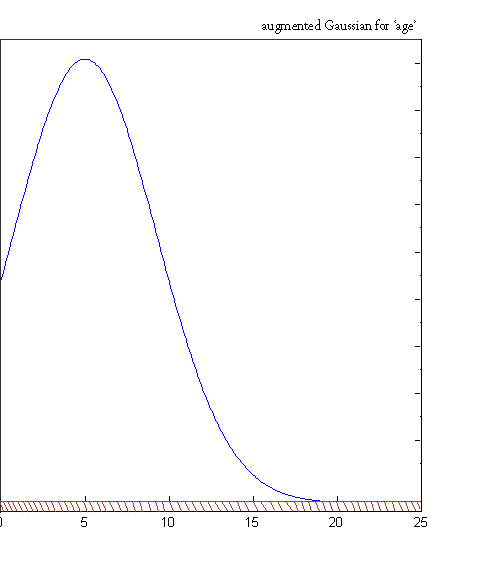
\includegraphics[scale=0.55]{img/AgeRegress2.png} 
\caption{Bootstrapping numeric feature values}
\end{figure}
\end{landscape}




%-------------------------------------------------------------------------------------------------------------------
% IMPLICATIONS
%-------------------------------------------------------------------------------------------------------------------
\section{Implications}\label{rnb-implication}
As a logical result of NBS, obtained samples will follow a different distribution than the ones obtained by (regular) bootstrapping. This idea is illustrated in figure~\ref{fig:NBS}, and in the following example. Assume a minority dataset $Z$ which is described by a binary class $Y$ and two binary features ($X_1$ and $X_2$), such that $Z = X_1 \times X_2 \times Y$:

\begin{table}[h]
\centering  
\begin{tabular}{ c c c}    
Feature 1 & Feature 2 & Class Label\\
\hline
1& 1& 1\\
1& 0& 1\\
0& 1& 0\\
0& 0& 1\\
1& 1& 1\\
1& 0& 0\\
0& 0& 0\\
1& 0& 0\\
\end{tabular}
\label{tab:exampleZ}
\caption{A possible minority dataset $Z$} % title name of the table
\end{table}

If we consider the sampling schemes (1) NBS and (2) bootstrapping, we can say the following:

\begin{itemize}
\item In (1), feature values are bootstrapped independently from $X_1$ and $X_2$ such that $P(X_1)$ and $P(X_2)$ become independent in the samples:
\begin{eqnarray}
P(X_1 \wedge X_2) &=& P(X_1 \cap X_2) \nonumber \\
&=& P(X_1|X_2)\;P(X_2) \nonumber \\
&=& P(X_1)\;P(X_2) \label{eq:px1px2indep}
\end{eqnarray}
\item In (2), instances are bootstrapped from $Z$ such that $P(X_1 \wedge X_2)$ is more or less preserved in the samples. This also means that feature dependencies are remained in the samples, such that:
\begin{eqnarray}
P(X_1 \wedge X_2) &=& P(X_1 \cap X_2) \nonumber \\
&=& P(X_1|X_2)\;P(X_2) \label{eq:px1px2dep} \\
&\neq& P(X_1)\;P(X_2) \nonumber
\end{eqnarray}
\end{itemize}

If we repeat the sampling process multiple times by creating a bagging ensemble, the distributions of $P(X_1)$ and $P(X_2)$ behave as random variables. In (1), these disributions will be independent, while in (2) these distributions will be correlated. Although a Naive Bayes classifier does not consider the feature dependencies present in the training data, we explain how existing correlations influence the variance of the estimates in a Naive Bayes classifier. The decision boundary for $Y$ in Naive Bayes is given as:

\begin{eqnarray}
Y &\longleftarrow& \mbox{arg max $y$ }\;\frac{\hat{P}(Y = y) \prod_{i=1}^m{\hat{P}(X_i|Y=y)}}{\sum_{j=1}^{|Y|}{\hat{P}(Y=y_j)} \prod_{i=1}^{m}{\hat{P}(X_i|Y=y)}} \label{eq:naivebayesdenom}\\
&\longleftarrow& \mbox{arg max $y$ }\;\hat{P}(Y = y) \prod_{i=1}^m{\hat{P}(X_i|Y=y)}\label{eq:naivebayesnodenom}
\end{eqnarray}

Equation~\ref{eq:naivebayesnodenom} allows us to calculate the variance over the estimates of $Y$ when we construct a bagging ensemble of Naive Bayes classifiers using sampling schemes (1) and (2). Please note that the expression $\sum_{j=1}^{|Y|}{\hat{P}(Y=y_j)} \prod_{i=1}^{m}{\hat{P}(X_i|Y=y)}$ differs in sampling scheme (1) and (2), as the estimates come from a different distribution.  However, for sake of simplicity we assume that this difference can be neglected \footnote{In figure~\ref{fig:varab} and \ref{fig:varabss100}, we can see that this simplification does not alter the type of relationship between the covariance of the prior probabilities and $\mbox{Var}\big(\hat{P}(Y=y|x)\big)$.} and continue from equation~\ref{eq:naivebayesnodenom}:

\begin{eqnarray}
\mbox{Var}\big(\hat{P}(Y=y|x)\big) &\propto& Var \big (\hat{P}(Y = y) \prod_{i=1}^m{\hat{P}(X_i|Y=y)} \big )\label{eq:varNBfull}
\end{eqnarray}

Since both in (1) and (2) we have that $P(Y = y)$ is a constant that represents the likelihood of the class $y$, we can rewrite equation~\ref{eq:varNBfull} as follows:

\begin{eqnarray}
\mbox{Var}\big(\hat{P}(Y=y|x)\big) &\propto& \mbox{Var} \big (\prod_{i=1}^m{\hat{P}(X_i|Y=y)} \big )
\end{eqnarray}

If we consider a dataset which is described by two features $X_1$ and $X_2$, we can rewrite previous equation as:

\begin{eqnarray}
\mbox{Var}\big(\hat{P}(Y=y|x)\big)) &\propto& \mbox{Var} \big (\hat{P}(X_1|Y=y)\, \hat{P}(X_2|Y=y)\big )\label{eq:nbsimplified}
\end{eqnarray}

Since $\hat{P}(X_1|Y=y)$ and $\hat{P}(X_2|Y=y)$ are random variables, we need to know how we can work out the variance of their product. As expressed by Goodman~\cite{exactvar60}, the variance of a product of two random variables $a$ and $b$ is equal to:

\begin{eqnarray}
\mbox{Var}(ab) &=& A^2\,\mbox{Var}(b) + B^2\,\mbox{Var}(a) + 2ABE_{11} \nonumber \\
&& + 2AE_{12} + 2BE_{21} + E_{22} - E_{11}^2\label{eq:varxy}\\
&\approx& A^2\,\mbox{Var}(b) + B^2\,\mbox{Var}(a) + 2ABE_{11}\label{eq:varxyapprox}
\end{eqnarray}

where 

\begin{itemize}
\item $A = E(a)$ : the expected value of $a$
\item $B = E(b)$ : the expected value of $b$
\item $E_{ij} = E\ \big ((a-A)^i (b-B)^j\big )$
\end{itemize}

Often, Var($ab$) is approximated by equation~\ref{eq:varxyapprox}. Since by definition $\mbox{Cov}(a,b) = E \big ( (a-E(a))(b-E(b) \big )$, we can say that $E_{11}$ is the covariance between $a$ and $b$. When feature independence holds, we can say the following:

\begin{eqnarray}
E(ab) &=& E(a)\;E(b)
\end{eqnarray}

and therefore:
\begin{eqnarray}
E \big ( (a + Ct_1) (b + Ct_2) \big ) &=& E (a + Ct_1)\; E(b + Ct_2)
\end{eqnarray}

This means that when feature independence holds, we can simplify equation~\ref{eq:varxy} as follows:

\begin{eqnarray}
\mbox{Var}^I(ab) &=& A^2\,\mbox{Var}(b) + B^2\,\mbox{Var}(a) + 2ABE_{11} + 2AE_{12} + 2BE_{21} + E_{22} - E_{11}^2 \nonumber \\
&=& A^2\,\mbox{Var}(b) + B^2\,\mbox{Var}(a) + 2ABE \big ((a-A) (b-B) \big) \nonumber \\
&& + 2AE \big ((a-A) (b-B)^2 \big ) + 2BE \big ((a-A)^2 (b-B) \big ) \nonumber \\
&& + E \big ((a-A)^2 (b-B)^2 \big ) - E^2 \big ((a-A) (b-B) \big )\nonumber \\
&=& A^2\,\mbox{Var}(b) + B^2\,\mbox{Var}(a) + 2ABE (a-A) \,E (b-B) \nonumber \\
&& + 2AE (a-A) \,E \big ( (b-B)^2 \big ) + 2BE \big ((a-A)^2 \big ) \,E(b-B) \nonumber \\
&& + E \big ((a-A)^2 \big ) \, E \big ((b-B)^2 \big ) - E(a-A)E(a-A)\,E(b-B)E(b-B) \nonumber \\
\nonumber \\
&& \mbox{where $E(a-A) = E(a)-E(A) = E(a) - E(E(a)) = E(a) - E(a) = 0$} \nonumber\\
&& \mbox{and similartly $E(b-B) = 0$} \nonumber\\
\nonumber \\
&=& A^2\,\mbox{Var}(b) + B^2\,\mbox{Var}(a) + E \big ((a-A)^2 \big) \, E \big ( (b-B)^2 \big) \nonumber \\
&=& A^2\,\mbox{Var}(b) + B^2\,\mbox{Var}(a) + \mbox{Var}(a)\mbox{Var}(b) \label{eq:varxyindep}
\end{eqnarray}

As a result,

\begin{eqnarray}
\mbox{Var}(ab) &=& \mbox{Var}^I(ab) + 2ABE_{11} + 2AE_{12} + 2BE_{21} - E_{11}^2 \nonumber \\
&& -\mbox{Var}(a) \mbox{Var}(b) + E_{22} \label{eq:indepvsdep}\\
&\approx& \mbox{Var}^I(ab) + 2ABE_{11} -\mbox{Var}(a) \mbox{Var}(b)
\end{eqnarray}

of which $2ABE_{11} -\mbox{Var}(a) \mbox{Var}(b)$ is the biggest term besides $\mbox{Var}^I(ab)$ due to the often accepted approximation as expressed in equation~\ref{eq:varxyapprox}. Using this equation, we can calculate how the variance of $ab$ will differ when $a$ and $b$ are independent or correlated:

\begin{eqnarray}
\mbox{Var}(ab) - \mbox{Var}^I(ab) &=&  2ABE_{11} + 2AE_{12} + 2BE_{21} - E_{11}^2 \nonumber \\
&& -\mbox{Var}(a) \mbox{Var}(b) + E_{22}\label{eq:diffdepindep} \\
&\approx&  2ABE_{11} -\mbox{Var}(a) \mbox{Var}(b) \label{eq:diffdepindepapprox} 
\end{eqnarray}

Previous equation shows that the covariance between $a$ and $b$ (which is expressed by $E_{11}$) plays an important role in how the variance of $ab$ will change. However, because other terms as well also play a role in this difference, it is hard to make any general statements about the outcome of expression~\ref{eq:diffdepindep}. For this reason, we analyse the effect of different covariances between $a$ and $b$ on $\mbox{Var}(ab)$.






\newpage
We can distinguish three types of possible correlations between $a$ and $b$ such that:

\begin{enumerate}
\item $a$ and $b$ are dependent on each other, such that $\mbox{Cov}(a,b) < 0$
\item $a$ and $b$ are independent from each other, such that $\mbox{Cov}(a,b) = 0$
\item $a$ and $b$ are dependent on each other, such that $\mbox{Cov}(a,b) > 0$
\end{enumerate}

\begin{figure}[htp]
\centering
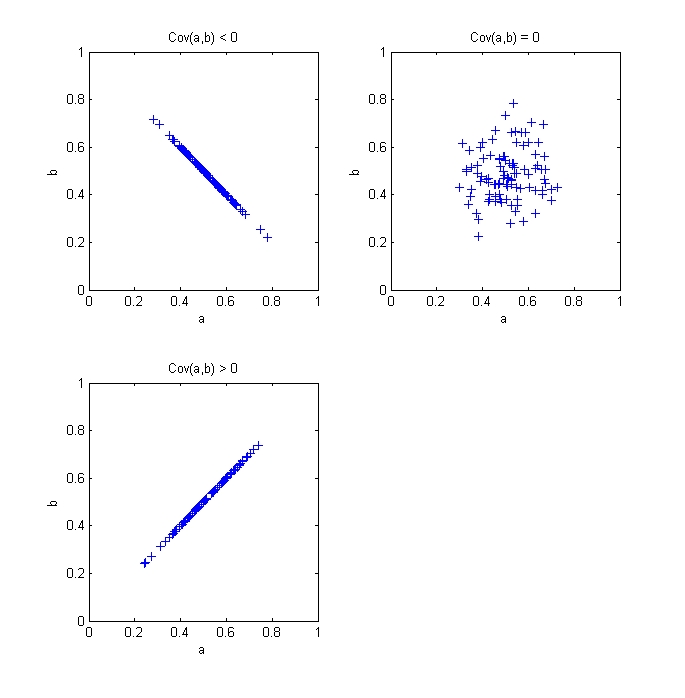
\includegraphics[scale=0.60]{img/correlations.png}
\caption{Three types of correlations between $a$ and $b$}
\end{figure}

\newpage
We can now measure what happens with Var($ab$) when $\mbox{Cov}(a,b) \neq 0$ (thus, when $a$ and $b$ are dependent). Figure~\ref{fig:varab} illustrates that when Cov($a,b$) rises, so does Var($ab$). Also, it is clear that this relation can be approximated by a linear function, as long as the sample sizes of $a$ and $b$ are big enough (see figure~\ref{fig:varabss100}).

\begin{figure}[h]
\centering
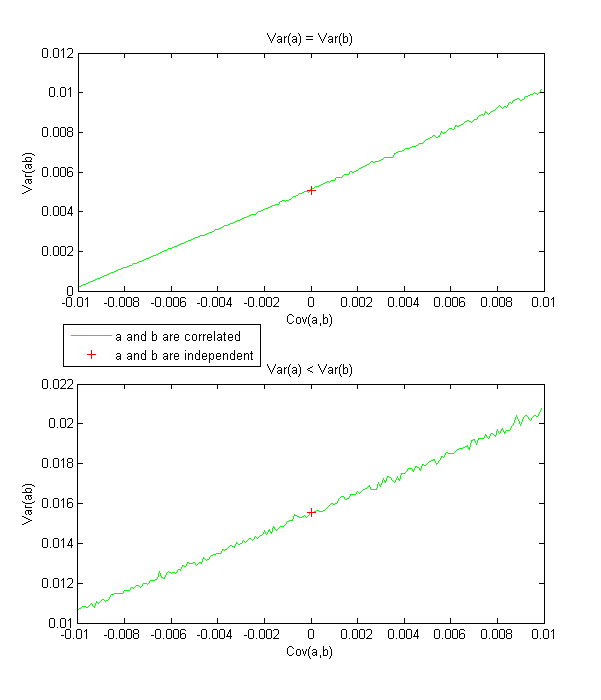
\includegraphics[scale=0.70]{img/varabss50000.png}
\caption{The effect of covariance between $a$ and $b$ on Var($ab$) (sample size: 50\,000)}
\label{fig:varab}
\end{figure}

\newpage
\begin{figure}[h]
\centering
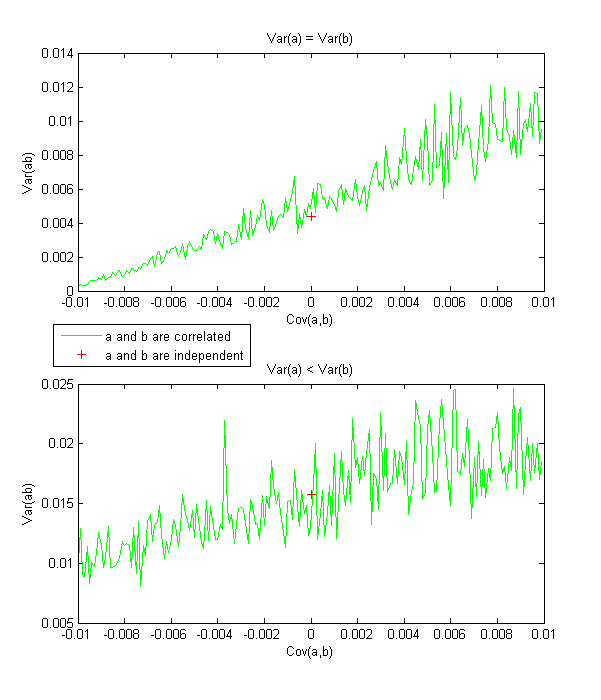
\includegraphics[scale=0.70]{img/varabss100.png}
\caption{The effect of covariance between $a$ and $b$ on Var($ab$) when the size of the samples is small (sample size: 100)}
\label{fig:varabss100}
\end{figure}

If we consider again expression~\ref{eq:nbsimplified}, we can say that:

\begin{itemize}
\item $a=\hat{P}(X_1|Y=y)$
\item $b=\hat{P}(X_2|Y=y)$
\end{itemize}

such that

\begin{eqnarray*}
\mbox{Var}(ab)&=&\mbox{Var}\big(\hat{P}(Y=y|x)\big)\\
&\propto& \mbox{Var}\big( \hat{P}(X_1|Y=y)\,\hat{P}(X_2|Y=y)\big)
\end{eqnarray*}
Based on figure~\ref{fig:varab} and \ref{fig:varabss100}, we can expect that when the prior estimates $\hat{P}(X_1|Y=y)$ and $\hat{P}(X_2|Y=y)$ have a positive (negative) covariance, the variance of $\hat{P}(Y=y|x)$ will increase (decrease). This expectation is also expressed in equation~\ref{eq:diffdepindepapprox}, which approximates the relation between Cov$\big (\hat{P}(X_1|Y=y),\hat{P}(X_2|Y=y)\big)$ and Var$\big (\hat{P}(X_1|Y=y)\,\hat{P}(X_2|Y=y)\big)$. However, when the sample size of $\hat{P}(X_1|Y=y)$ and $\hat{P}(X_2|Y=y)$ (and therefore the size of the bagging ensemble) is not very large, this relation becomes very unreliable. This effect is illustrated in figure~\ref{fig:varabss100}.  If we translate these observations to sampling schemes (1) NBS and (2) bootstrapping, we can make the following statements. In sampling scheme (2), we know that random variables $\hat{P}(X_1|Y=y)$ and $\hat{P}(X_2|Y=y)$ are not independent, and that the estimates of the dependencies are unreliable when there is a lack of training data. We showed that Naive Bayes Sampling removes all feature dependencies, with the result that the \textbf{variance} of $\hat{P}(Y=y|x)$ will decrease (increase) when the covariance between $\hat{P}(X_1|Y=y)$ and $\hat{P}(X_2|Y=y)$  in the original dataset is positive (negative). This means that if we have positive covariance, we better follow the independence sampling scheme (1) in order to reduce the variance of our (test) predictions. Now, if the two features are indeed dependent, introducing artificial independence has an effect on the \textbf{bias} of the prediction error as well. In a Naive Bayes classifier, the bias of the estimate $\hat{P}(Y=y|x)$ is given by:
\begin{eqnarray}
\mbox{Bias}\,(\hat{P}(Y=y|x)) = E(\hat{P}(Y=y|x)) - P(Y=y|x)\label{eq:bias}
\end{eqnarray}
It should be clear that the outcome of $E(\hat{P}(Y=y|x))$ is different when we apply Naive Bayes Sampling and Bootstrapping on a dataset that is not feature independent. Since we do not know $P(Y=y|x)$, it is hard to predict for what sampling scheme and under what conditions the bias, as given in expression~\ref{eq:bias}, will be smaller. 
 What we do know is that in some situations, the variance of the estimate decreases when we apply Naive Bayes Sampling. Hence, in order to choose between Naive Bayes Sampling and Bootstrapping, we advise comparing both techniques and to choose that implementation which results into a better performance on the considered dataset.
 
Although the exact impact of Naive Bayes Sampling is not clear, we can motivate its use as follows. We know that the independence assumptions on which Naive Bayes classifiers are based, almost never hold for natural data sets. Because of this reason, machine learning and information retrieval focused on three kind of strategies~\cite{lewis98}: (1) attempts to produce better classifiers by relaxing the independence assumption, (2) modifications of the features to make the independence assumption more true, and (3) attempts to explain why the independence assumption isn't really needed anyway.

Clearly, Naive Bayes Sampling implements the second strategy by imposing feature independency on the dataset. Other approaches that implement this strategy can mainly be found in information retrieval~\cite{booleanqueries}~\cite{bayesianinference}~\cite{harper78eval}~\cite{Turtle91evaluationof}~\cite{Rijsbergen77}.   
Up to this moment, the effectiveness improvements yielded by these approaches is rather small. Moreover, the nature of their impact is more complex than might be guessed~\cite{Church95oneterm}. The implications of Naive Bayes Sampling illustrate this problem. As a result, we show the performance of Naive Bayes Sampling by a number of experiments in chapter~\ref{experiments}. In order to obtain a full understanding in the differences between Naive Bayes Sampling and Bootstrapping, more research is required.


\begin{figure}[h]
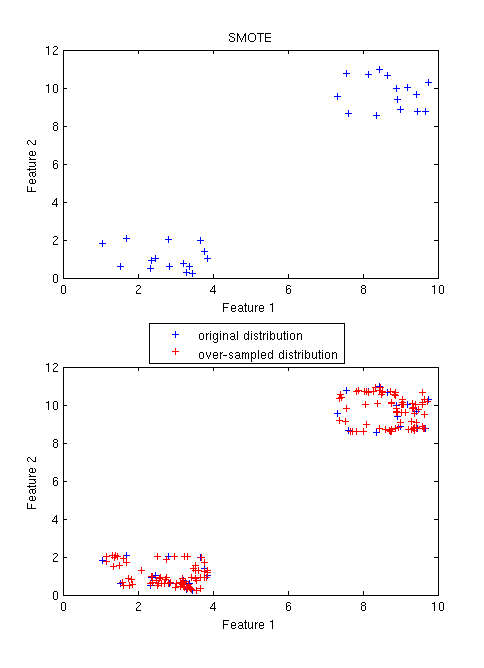
\includegraphics[scale=0.65]{img/SMOTE_featureSampling.png}
\caption{This figure shows how SMOTE emphasizes the generation of synthetic examples within existing minority clusters. The parameter $k$ influences how strict these clusters have to be interpreted, and therefore also the generalization process of the learning algorithm. In the first image, a possible 2-dimensional minority distribution is displayed. This distribution clearly shows two clusters of minority instances, namely one in the bottom left corner, and one in the top right corner. In the second image, the same distribution is displayed (blue), together with an over-sampled distribution by applying the SMOTE technique (red).}
\label{fig:SMOTE}
\end{figure}

\begin{figure}[h]
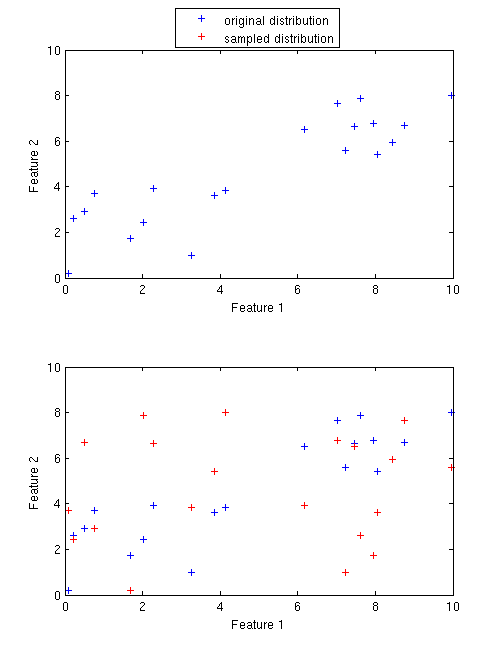
\includegraphics[scale=0.75]{img/nb_featureSampling.png}
\caption{This figure illustrates the effect of sampling with the introduced sampler in section~\ref{rnb-approach}. In the first image, a possible 2-dimensional minority distribution is displayed. This distribution clearly shows two clusters of minority instances, namely one in the bottom left corner, and one in the top right corner. In the second image, the same distribution is displayed (blue), together with a possible synthetic over-sampled distribution (red). This distribution however does not form two clusters anylonger, and is scattered over the joint distribution of the feature space.}
\label{fig:NBS}
\end{figure}




\section{Conclusion}\label{rnb-conclusion}
Experiment results in section~\ref{exp-rnb} show that the introduced approach (RNB-FvB) clearly outperforms current approaches to class imbalance, especially when the datasets contain a large amount of nominal features. Although it is hard to predict how the bias changes when applying RNB-FvB, previous section showed that a positive covariance between the features decreases the variance. As a result, RNB-FvB allows to increase the stability of bagging ensembles when the features have a positive covariance. In order to know when Naive Bayes Sampling outperforms Booststrapping, we advise comparing both techniques by means of stratified 10-fold cross-validation.

Despite of the many benefits, some backdraws hinder the implementation of RNB-FvB. First of all, the sampling process consumes a lot of time (and memory), especially due to the implemented EM-algorithm for numeric features. When a high number of samples needs to be created, it might therefore be more appropriate to undersample the majority class first. A second problem relates to the fact that the introduced sampler can only successfully be implemented with a Naive Bayes classifier (due to the imposed feature independence). This restriction however logically follows from the applied sampling scheme NBS, which is exactly developed to improve cooperation with a Naive Bayes classifier. 

Hence, the restrictions of NBS allow to improve the stability and reliability of a bagging ensemble of Naive Bayes classifiers (RNB-FvB). Also, it is clear that not only all assumptions in this ensemble meet each other, but are moreover validated (due to the imposition of feature independence). This is probably the main reason why RNB-FvB outperforms techniques like cost-sensitivity, SMOTE, Bagging for Imbalanced Datasets and MetaCost.





